\section{Backend}
\label{sec:backend}

Nel capitolo seguente verrà descritto in maniera più approfondita il modulo \textit{backend}, ovvero il modulo che si occupa di gestire le richieste provenienti dal \textit{frontend} filtrando i dati presenti nella blockchain e nel database. Il modulo è stato sviluppato utilizzando il linguaggio di programmazione \textit{python} ed il framework \textit{Django}. 

È importante sottolineare che sebbene avere un server di \textit{backend} possa sembrare in contrasto con il principio di decentralizzazione, la sua presenza è fondamentale per ottimizzare i tempi di risposta e fornire agli utenti un'esperienza d'uso migliore.  Inoltre, come si potrà notare nel capitolo, il \textit{backend} ha il solo scopo di essere da tramite e filtro tra il \textit{frontend} e la blockchain.

\subsection{API}

Lo scopo principale del modulo \textit{backend} è quello di fornire delle \textit{Application programming interface} (API) al \textit{frontend} con i dati necessari per la visualizzazione delle informazioni. In particolare, le API devono permettere di recuperare le informazioni relative ad un asset, ad una collezione e ad un utente. Inoltre, devono permettere di recuperare le informazioni relative alle vendite in corso presenti sul marketplace. Per offrire le funzionalità appena descritte, è stato deciso di utilizzare \textit{GraphQL}\footnote{https://graphql.org/}, un linguaggio di \textit{query} API alternativo a \textit{REST}.

Di seguito è possibile vedere un esempio di \textit{query} GraphQL per recuperare le informazioni degli asset posseduti da un utente. Si noti come sia possibile specificare quali informazioni si vogliono ricevere in risposta, in questo caso il nome, l'indirizzo del contratto e l'identificativo dell'asset. Seppure nell'API progettata sia possibile richiedere anche altre informazioni come l'immagine e i metadati.

\begin{lstlisting}[basicstyle=\small]
    query {
        ownedNfts(address: "0x...") {
            contractAddress
            tokenId
            name
        }
    }
\end{lstlisting}

Il framework \textit{Django} permette la creazione di \textit{app}, ovvero moduli interni che consentono una maggiore modularità e organizzazione del codice. Quando configurato con \textit{GraphQL}, ogni \textit{app} genera automaticamente uno \textit{schema}, ossia un insieme di \textit{query} e \textit{mutation}. Le \textit{query} sono funzioni che permettono di recuperare i dati, mentre le \textit{mutation} permettono di modificarli. In particolare, le \textit{mutation} sono utilizzate per interagire con il database.

Con la configurazione di base di \textit{Graphene}\footnote{https://graphene-python.org/} (libreria con lo scopo di semplificare l'integrazione di \textit{GraphQL}), ogni \textit{app} genera un proprio URI nel quale è possibile effettuare le richieste. 

Per semplificare l'implementazione e l'interazione con le API è stato deciso di implementare il concetto di \textit{Federation schema}. Esso permette di creare uno schema unico che contiene tutte le \textit{query} e le \textit{mutation} disponibili, mantenendo comunque la modularità del codice. In questo modo, è possibile effettuare una singola richiesta per recuperare i dati da più \textit{app} differenti.

Entrando più nel dettaglio nell'implementazione effettuata, il \textit{backend} è composto da tre \textit{app} differenti:

\begin{itemize}
    \item \textit{BlockchainAPI}: Si occupa di recuperare i dati dalla blockchain, specialmente i dati relativi a collezioni, asset ed eventi.
    \item \textit{MarketplaceAPI}: Recupera tutte le informazioni relative al marketplace.
    \item \textit{databaseAPI}: Interagisce con il database, in particolare con i dati relativi all'utente.
\end{itemize}

La figura \ref{fig:federationSchema} rappresenta lo schema delle API, in particolare è possibile notare il funzionamento del \textit{Federation schema} e del modulo \textit{backend}.

\begin{figure}[H]
    \centering
    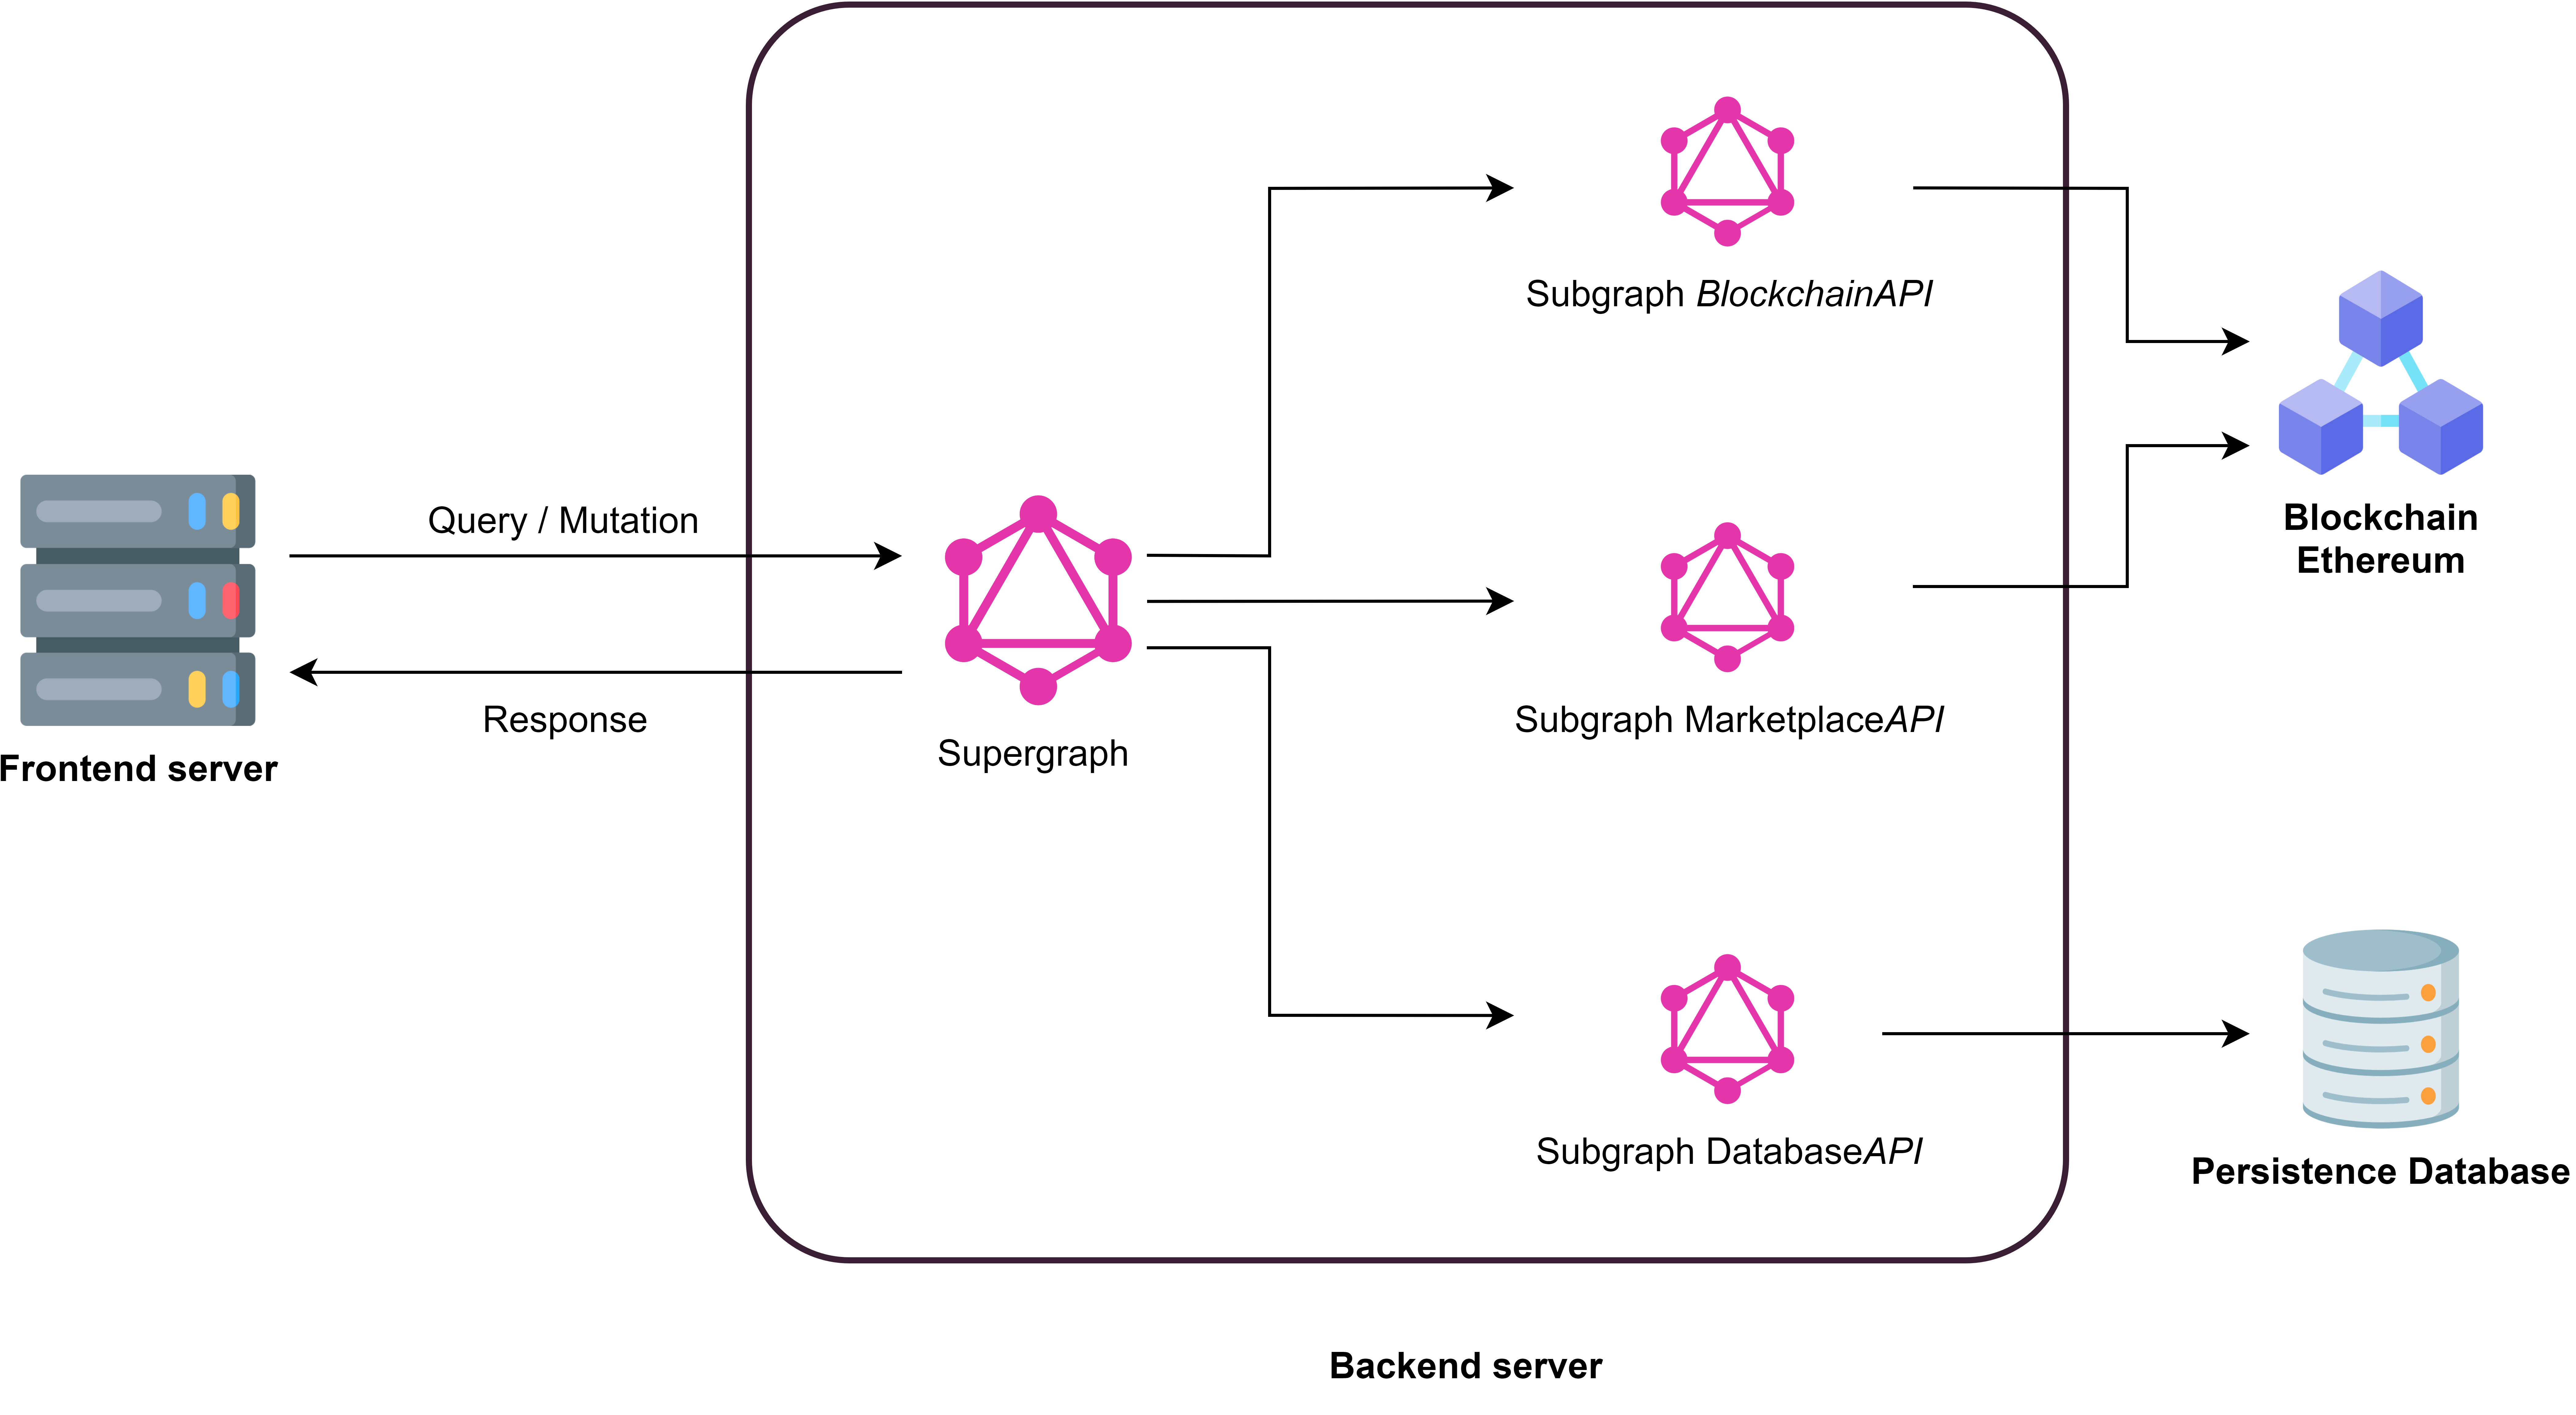
\includegraphics[width=1\textwidth]{images/GraphQLFederationSchema.png}
    \caption{Schema delle API}
    \label{fig:federationSchema}
\end{figure}

All'interno dei prossimi capitoli verranno analizzate le \textit{query} e le \textit{mutation} disponibili nelle tre \textit{app}.

\subsubsection{Blockchain API}

All'interno del \textit{subgraph Blockchain API} sono presenti diverse query che permettono di recuperare le informazioni presenti nella blockchain. Come descritto nel capitolo \hyperref[sec:recuperoDatiBlockchain]{\textit{Recupero dei dati dalla blockchain}} è possibile recuperare i dati di una collezione solamente se si conosce l'indirizzo del contratto che la rappresenta.
Di seguito è presente una lista delle principali \textit{query} disponibili, con il relativo scopo e funzionamento.

\begin{itemize}
    \item \textit{ownedNfts}: Recupera tutti gli asset posseduti da un utente specifico. filtrando gli eventi \textit{Transfer} presenti negli smart contracts da lui osservati.
    \item \textit{nftComplete}: Recupera tutte le informazioni relative ad un asset, contattando lo smart contract e analizzando i metadati su IPFS.
    \item \textit{collection}: Ritorna le informazioni di una collezione e tutti gli asset presenti al suo interno, contattando lo smart contract e filtrando gli eventi di \textit{Transfer} in base alla tipologia (\textit{Mint} o \textit{Burn}).
    \item \textit{contract}: Risolve unicamente le informazioni base di un contratto. Ovvero il nome, il simbolo e l'indirizzo.
    \item \textit{nftHistory}: Analizzando gli eventi di trasferimento, approvazione e relativi al marketplace di un asset, ritorna la cronologia completa di un asset.
    \item \textit{royaltyCollection}: Contattando il contratto della collezione, recupera le informazioni riguardanti le royalty di default per una collezione, ritornando la compatibilità con lo standard ERC2981 e/o ERC2981MultiReceiver, nonchè la percentuale per ogni ricevente.
    \item \textit{withdrawRoyaltyCollection}: Nel caso in cui la collection possieda un PaymentSplitter, ritorna l'ammontare che è possibile prelevare.
    \item \textit{royaltyToken} e \textit{withdrawRoyaltyToken}: Come le \textit{query} precedenti, ma per un singolo asset.
    \item \textit{collectionOwner}: Verifica che l'indirizzo passato come parametro sia il proprietario di una collezione, anch'essa passata come parametro. Questa \textit{query} è utilizzata per verificare che l'utente abbia il diritto di accedere alla pagina di gestione di una collezione.
    \item \textit{contractOwnedCreatedWithShopychange}: Come descritto nel capitolo \hyperref[sec:creazioneNFT]{\textit{Creazione NFT}}, questa \textit{query} ritorna gli indirizzi di collezioni creati tramite Shopychange.
\end{itemize}

\subsubsection{Marketplace API}

L'\textit{app Marketplace API} si occupa di recuperare le informazioni relative al marketplace. All'interno dello schema sono presenti le seguenti \textit{query}:

\begin{itemize}
    \item  \textit{sales}: Recupera tutte le vendite in corso presenti sul marketplace, contattando il metodo all'interno del contratto \textit{MarketplaceFundamental}.
    \item \textit{sale}: Ottiene le informazioni di vendita di uno specifico token.
    \item \textit{isMarketplaceApproved}: Verifica che il marketplace sia approvato per la gestione di un asset.
    \item \textit{isTokenForSale}: Verifica che un asset sia in vendita.
    \item \textit{marketplaceRoyalty}: Recupera la percentuale di revenue share che il marketplace richiede per ogni vendita.
    \item \textit{marketplaceBalace}: Ottiene il bilancio del marketplace ottenuto tramite il revenue share.
\end{itemize}

\subsubsection{Database API}

Lo schema \textit{Database API} presenta le \textit{query} e \textit{mutation} per recuperare e modificare i dati presenti nel database. Più nel dettaglio, i dati modificabili sono una lista di collezioni che l'utente vuole monitorare. Le \textit{query} e \textit{mutation} sono le seguenti:

\begin{itemize}
    \item \textit{ContractObserved}: Ritorna la lista di collezioni che l'utente vuole monitorare.
    \item \textit{AddUser}: Aggiunge un utente al database.
    \item \textit{AddNFTCollection}: Aggiunge una collezione alla lista di collezioni monitorate da un utente.
    \item \textit{AddNFTCollections}: Come la \textit{mutation} precedente, ma per più collezioni.
    \item \textit{RemoveNFTCollection}: Rimuove una collezione dalla lista di collezioni osservate da un utente.
    \item \textit{RemoveNFTCollections}: Come la \textit{mutation} precedente, ma per più collezioni.
\end{itemize}

\subsection{Database}

Il database è stato implementato utilizzando \textit{MongoDB}, un database non relazionale che permette di salvare i dati su documenti. Il database è stato collegato utilizzando la libreria \textit{djongo}\footnote{https://www.djongomapper.com/} che permette di connettere \textit{Django} con \textit{MongoDB}. Essendo che il progetto sviluppato è una \textit{dApp}, le informazioni da salvare sono poche e non fondamentali per il funzionamento del sistema. Infatti, l'unica informazione salvata sul database è la lista di collezioni che l'utente ha deciso di osservare. In aggiunta, è presente una tabella che contiene una lista di collezioni generiche che tutti gli utenti monitorano, l'obiettivo è di permettere agli utenti di visualizzare le collezioni più popolari senza doverle cercare manualmente.

\subsection{Test}

Tutte le query e mutation presenti nel \textit{Federation schema} sono completamente testate utilizzando il \textit{tool} già integrato in \textit{Django}. I test verificano che i dati vengano filtrati, elaborati e restituiti correttamente sia in caso di parametri validi che non validi. Inoltre, sono stati implementati dei test per verificare la giusta gestione degli errori in caso di valori non previsti restituiti dalla blockchain e dal database.

\subsection{Motivazioni e Alternative}

Le alternative a livello di linguaggio di programmazione e framework sono molteplici, la sceltà è però da ricondurre alle librerie di connessione con la blockchain in quanto sono meno numerose. Di queste, le più famose e utilizzate sono:

\begin{itemize}
    \item \textit{Web3.js}\footnote{https://web3js.readthedocs.io/}: Libreria JavaScript/TypesScript
    \item \textit{Web3.py}\footnote{https://web3py.readthedocs.io/}: Libreria Python
    \item \textit{Ethers.js}\footnote{https://docs.ethers.org/v5/}: Libreria JavaScript/TypesScript
\end{itemize}

Essendo il \textit{frontend} sviluppato utilizzando \textit{Typescript}, come definito dai requisiti del progetto. La scelta è ricaduta su \textit{Web3.py} così da ampliare le conoscenze e competenze in ambito di sviluppo Python. 

Pertanto, avendo conoscenze ridotte nell'ambito Python è stato deciso di utilizzare il framework \textit{Django}, in quanto è uno dei più utilizzati e ricco di documentazione. Una possibile alternativa è \textit{Flask}\footnote{https://flask.palletsprojects.com/}.

La decisione che ha portato all'adozione di API di tipo GraphQL, quindi non API di tipo REST, è stata presa in quanto offrono maggiore flessibilità ed efficienza. Più in dettaglio, tramite il linguaggio \textit{query} utilizzato da GraphQL è possibile richiedere informazioni da più \textit{app}/\textit{endopoint} in una singola richiesta. Inoltre, GraphQL permette di definire quali informazioni si vogliono ricevere in risposta, in questo modo è possibile ridurre il traffico di rete e il tempo di risposta ma senza dover implementare nuove \textit{query}.

Infine, GraphQL presenta un sistema di \textit{cache} che permette di ridurre ulteriormente il tempo di risposta, in quanto è possibile salvare in cache le risposte alle richieste più frequenti. Tuttavia, quest'ultima funzionalità è stata disabilitata così da ottenere sempre le informazioni dalla blockchain più aggiornate ed evitare problemi di inconsistenza dei dati.
